\documentclass[tikz,border=10pt]{standalone}
\usepackage{tikz}
\usetikzlibrary{positioning}
\begin{document}
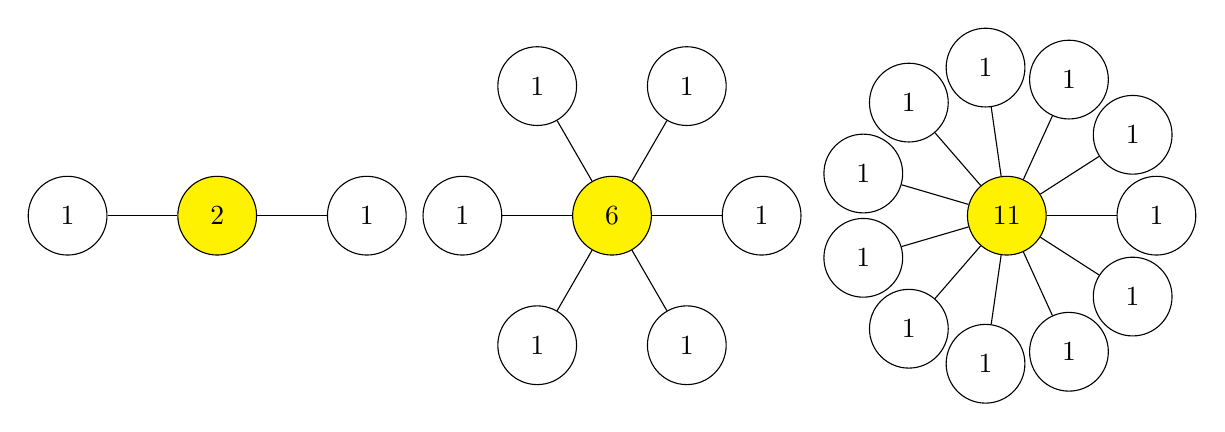
\begin{tikzpicture}[every node/.style={circle,draw,minimum size=1cm}]

% Left network with 3 nodes
\node[fill=yellow] (l-hub) at (0,0) {2};
\foreach \a [count=\i] in {0,180} {
  \node[fill=white] (l-spoke-\i) at ([shift={(\a:1.9cm)}]l-hub) {1};
  \draw (l-hub) -- (l-spoke-\i);
}

% Middle network with 6 nodes
\node[fill=yellow,right=4cm of l-hub] (m-hub) {6};
\foreach \a [count=\i] in {0,60,...,300} {
  \node[fill=white] (m-spoke-\i) at ([shift={(\a:1.9cm)}]m-hub) {1};
  \draw (m-hub) -- (m-spoke-\i);
}

% Right network with 11 nodes
\node[fill=yellow,right=4cm of m-hub] (r-hub) {11};
\foreach \a [count=\i] in {0,32.727,...,359} {
  \node[fill=white] (r-spoke-\i) at ([shift={(\a:1.9cm)}]r-hub) {1};
  \draw (r-hub) -- (r-spoke-\i);
}

\end{tikzpicture}
\end{document}
